% titlepage-demo.tex
\documentclass{beamer}
\usepackage{graphicx}
\usepackage{tikz}
\usetikzlibrary{matrix}
% items enclosed in square brackets are optional; explanation below
\title{Verifying filesystems in ACL2}
\subtitle{Project report, CS380L Fall 2017}
\author{Mihir Mehta}
\institute{
  Department of Computer Science\\
  University of Texas at Austin\\[1ex]
  \texttt{mihir@cs.utexas.edu}
}
\date{07 December, 2017}

\addtobeamertemplate{navigation symbols}{}{%
    \usebeamerfont{footline}%
    \usebeamercolor[fg]{footline}%
    \hspace{1em}%
    \large \insertframenumber/\inserttotalframenumber
}

\begin{document}

%--- the titlepage frame -------------------------%
\begin{frame}[plain]
  \titlepage
\end{frame}

%--- the presentation begins here ----------------%

\begin{frame}{Why we need a verified filesystem}
  \begin{itemize}
  \item Modern filesystems have become increasingly complex, and so
    have the tools to analyse and recover data from them.
  \item It would be worthwhile to specify and formally verify, in the
    ACL2 theorem prover, the guarantees claimed by filesystems and
    tools.
  \item Work on this project started last year - since then I've built
    5 increasingly complex models.
  \item The plan is to model FAT32, adding features in every model and
    maintaining proofs of correctness.
  \end{itemize}
\end{frame}

\begin{frame}{File system models}
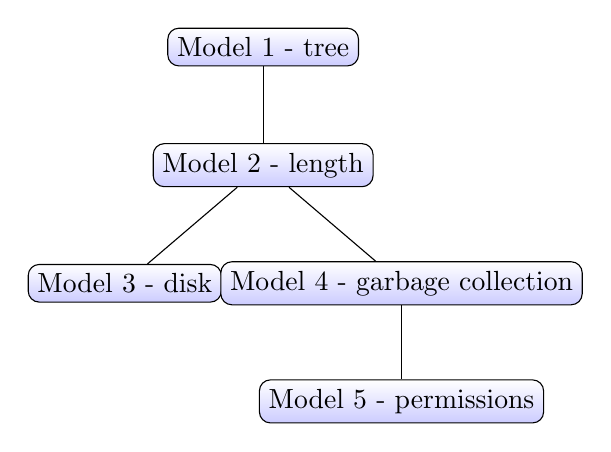
\begin{tikzpicture}[sibling distance=10em,
  every node/.style = {shape=rectangle, rounded corners,
    draw, align=center,
    top color=white, bottom color=blue!20}]
  \node {Model 1 - tree}
    child { node {Model 2 - length}
      child { node {Model 3 - disk}}
      child { node {Model 4 - garbage collection}
        child { node {Model 5 - permissions}}}};
\end{tikzpicture}
\end{frame}

\begin{frame}{Minimal set of operations?}
  \begin{itemize}
  \item The Google filesystem suggests a minimal set of operations:
    \begin{itemize}
    \item \texttt{create}
    \item \texttt{delete}
    \item \texttt{open}
    \item \texttt{close}
    \item \texttt{read}
    \item \texttt{write}
    \end{itemize}
  \item Of these, \texttt{open} and \texttt{close} require the
    maintenance of file descriptor state - so they can wait.
  \item However, they are essential when describing concurrency and
    multiprogramming behaviour.
  \item Thus, we can start modelling a filesystem, and several
    refinements thereof.
  \end{itemize}
\end{frame}

\begin{frame}{More about the models}
  \begin{itemize}
  \item Model 1: Tree representation of directory structure with unbounded
    file size and unbounded filesystem size.
  \item Model 2: Model 1 with file length as metadata.
  \item Model 3: Tree representation of directory structure with
    file contents stored in a "disk" (unbounded in length).
  \item Model 4: Model 3 with bounded filesystem size and garbage
    collection.
  \item Model 5: Model 4 with permissions for read/write for the user
    and others (no groups as yet)
  \end{itemize}
\end{frame}

\begin{frame}{Proof approaches and techniques}
  \begin{itemize}
  \item There are many properties that could be considered for
    correctness, but we choose to focus on the read-over-write
    theorems from the first-order theory of arrays.
  \item Read \texttt{n} characters starting at position \texttt{start}
    in the file at path \texttt{hns} in filesystem \texttt{fs}: \\
    \texttt{l1-rdchs(hns, fs, start, n)}
  \item Write string \texttt{text} characters starting at position \texttt{start}
    in the file at path \texttt{hns} in filesystem \texttt{fs}: \\
    \texttt{l1-wrchs(hns, fs, start, text)}
  \end{itemize}
\end{frame}
\begin{frame}[fragile]
  \frametitle{Proof approaches and techniques}
  \begin{itemize}
  \item The first read-over-write theorem defines the semantics of
    reading from a location after writing to the same
    location. Formally, assuming \texttt{n =
      length(text)} and suitable "type" hypotheses (omitted here): \\
\begin{verbatim}
  l1-rdchs(hns, l1-wrchs(hns, fs, start, text),
                 start, n) =
  text
\end{verbatim}
  \item The second read-over-write theorem defines the semantics of
    reading from a location after writing to a different
    location. Formally, assuming \texttt{hns1 != hns2} and suitable "type"
    hypotheses (omitted here):\\
\begin{verbatim}
  l1-rdchs(hns1, l1-wrchs(hns2, fs, start2, text2),
                 start1, n1) =
  l1-rdchs(hns1, fs, start1, n1)
\end{verbatim}
  \end{itemize}
\end{frame}

\begin{frame}{Proof approaches and techniques}
  \begin{itemize}
  \item For each of the models 1 through 5, we have proofs of correctness of
    the two read-after-write properties, making use of the proofs of
    equivalence between models and their successors.
  \item For model 5, the proof assumes the permissions are
    granted.
  \item The proof of the converse property - that reads and writes
    fail when permissions are not granted - remains to be done.
  \end{itemize}
\end{frame}

\begin{frame}{Proof example: first read-over-write in model 2}
  \begin{figure}
    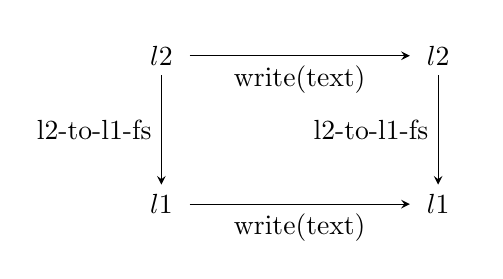
\begin{tikzpicture}
      \matrix (m) [matrix of math nodes,row sep=4em,column sep=8em,minimum width=2em]
              {
                l2 \pgfmatrixnextcell l2 \\
                l1 \pgfmatrixnextcell l1 \\};
              \path[-stealth]
              (m-1-1) edge node [left] {l2-to-l1-fs} (m-2-1)
              edge node [below] {write(text)} (m-1-2)
              (m-2-1.east|-m-2-2) edge node [below] {write(text)} (m-2-2)
              (m-1-2) edge node [left] {l2-to-l1-fs} (m-2-2);
    \end{tikzpicture}
    \caption{l2-wrchs-correctness-1}
  \end{figure}
  \begin{figure}
    \begin{tikzpicture}
      \matrix (m) [matrix of math nodes,row sep=4em,column sep=8em,minimum width=2em]
              {
                l2 \pgfmatrixnextcell text \\
                l1 \\};
              \path[-stealth]
              (m-1-1) edge node [left] {l2-to-l1-fs} (m-2-1)
              edge node [below] {read} (m-1-2)
              (m-2-1.east|-m-2-2) edge node [below] {read} (m-1-2);
    \end{tikzpicture}
    \caption{l2-rdchs-correctness-1}
  \end{figure}
\end{frame}

\begin{frame}{Proof example: first read-over-write in model 2}
  \begin{figure}
    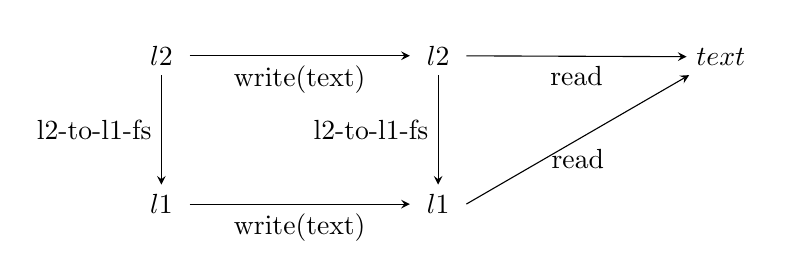
\begin{tikzpicture}
      \matrix (m) [matrix of math nodes,row sep=4em,column sep=8em,minimum width=2em]
              {
                l2 \pgfmatrixnextcell l2 \pgfmatrixnextcell text \\
                l1 \pgfmatrixnextcell l1 \\};
              \path[-stealth]
              (m-1-1) edge node [left] {l2-to-l1-fs} (m-2-1)
              edge node [below] {write(text)} (m-1-2)
              (m-2-1.east|-m-2-2) edge node [below] {write(text)} (m-2-2)
              (m-1-2) edge node [left] {l2-to-l1-fs} (m-2-2)
              edge node [below] {read} (m-1-3)
              (m-2-2.east) edge node [below] {read} (m-1-3);
    \end{tikzpicture}
    \caption{l2-read-over-write-1}
  \end{figure}
\end{frame}

\begin{frame}{Source analysis}
  \begin{table}[]
    \centering
    \caption{Code written for this project}
    \label{my-label}
    \begin{tabular}{ll}
      Source lines of code (ACL2)      & 6017 \\
      defun events (function definitions) & 118  \\
      defthm events (lemmas and proofs)   & 419 
    \end{tabular}
  \end{table}
\end{frame}

\end{document}
